% Experiment

\chapter{Experimental Setup}
\label{ch:experimental-setup}

For the experimentation phase we have used a Intel Core i7-6700HQ CPU
@ 2.60GHz, with 16GB of RAM, and a Cuda enabled Nvidia GeForce GTX
960M graphic card.

The data-set previously described in \autoref{part:variables} has been
pre-processed. This process consisted in narrowing down the data to
the same date range. Later the missing values where filled with
interpolated values. Finally the data-set has been normalized using a
standard score described in \autoref{eq:standard-score}.

\begin{equation}
  \begin{aligned}
    \label{eq:standard-score}
    X_{norm} & = \frac{X-\mu}{\sigma} \\
    X_{norm} & \leftarrow \text{Normalized instance}
    \\
    X & \leftarrow \text{Original instance}
    \\
    \mu & \leftarrow \text{Feature mean}
    \\
    \sigma & \leftarrow \text{Feature standard deviation}
    \\
  \end{aligned}
\end{equation}

After predicting the values of the BTC price, the values are still
normalized. In order to correctly interpret them and compute the error
measures, this prediction has been de-normalized using the inverse
function of \autoref{eq:standard-score}, which is represented in 
\autoref{eq:inverse-standard-score}.

\begin{equation}
  \begin{aligned}
    \label{eq:inverse-standard-score}
    \hat{X} & = \hat{X}_{norm} \times \sigma + \mu \\
    \hat{X}_{norm} & \leftarrow \text{Normalized prediction}
    \\
    \hat{X} & \leftarrow \text{De-normalized prediction}
    \\
    \mu & \leftarrow \text{Feature mean}
    \\
    \sigma & \leftarrow \text{Feature standard deviation}
    \\
  \end{aligned}
\end{equation}

After the pre-processing, and to avoid over-fitting we have used
\textit{time series cross-validation} proposed by
\cite{robjhyndman2010}. The particular implementation of this
technique used uses a test partition of size 1, which we call
$x_{t + 1}$ and a train partition composed of all the elements from
the $1095$-th to the $t$-th. The details about why we used $1095$-th
as the first element and the overall technique can be found in
\autoref{part:implementation}.

The layout of the network is the \textit{fully connected recurrent
  neural network} which is shown in \autoref{fig:rnn-topology}.

\begin{figure}[bth]
  \myfloatalign
  {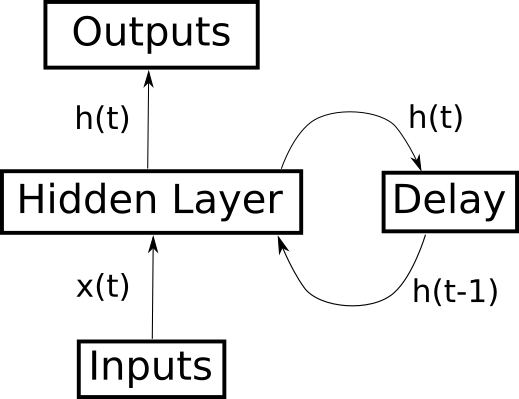
\includegraphics[width=.5\linewidth]
    {gfx/rnn-topology}}
  \caption{RNN topology.}
  \label{fig:rnn-topology}
\end{figure}

The first layer is composed of 1 neuron per instance, the hidden layer
is composed of another neuron per instances, and the output is
composed of only one neuron. More details related to RNNs can be found
in \autoref{part:method-technique}.


\chapter{Experimental Results}
\label{ch:experimental-results}

In this section we present the results of the experiments performed.
We decided that we would compare the performance of RNN with a
traditional method such as VAR.

Both \autoref{fig:predictions-subplots} and \autoref{fig:predictions}
represent a day ahead prediction of the Bitcoin price, compared to the
actual Bitcoin price, shown in the variable \textit{MarketPrice}. Is
the same information presented in two different ways to allow the
viewer to see the particular values of each one in
\autoref{fig:predictions-subplots}, and, on the other side, to be able
to compare closely the values of the two models and
\textit{MarketPrice} the viewer can use \autoref{fig:predictions}.

\begin{figure}[bth]
  \myfloatalign
  {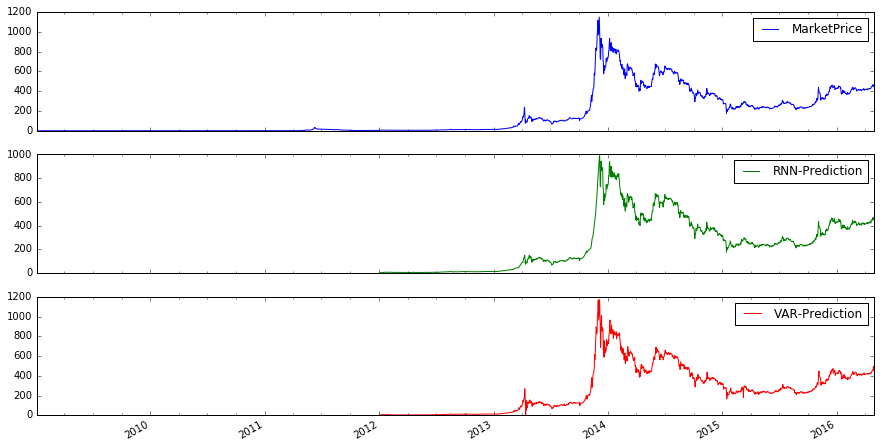
\includegraphics[width=1\linewidth]
    {gfx/predictions-subplots}}
  \caption{Predictions models and \textit{MarketPrice} true values in
    separate charts.}
  \label{fig:predictions-subplots}
\end{figure}

Although the shapes of the charts are similar, it can be noticed how
RNN takes more instances to learn certain patterns, like the one
present in the first quarter of 2013, where RNN doesn't have the spike
that VAR and \textit{MarketPrice} do have.

It can also be noticed in \autoref{fig:predictions} that RNN has a
delay compared to VAR and \textit{MarketPrice}. This can give as the
intuition that RNN learning rate is lower than VAR. But all this
observation are mere thoughts but are not a measure the correct
measure to quantify the goodness of prediction models and neither is a
suitable technique to compare prediction models.

\begin{figure}[bth]
  \myfloatalign
  {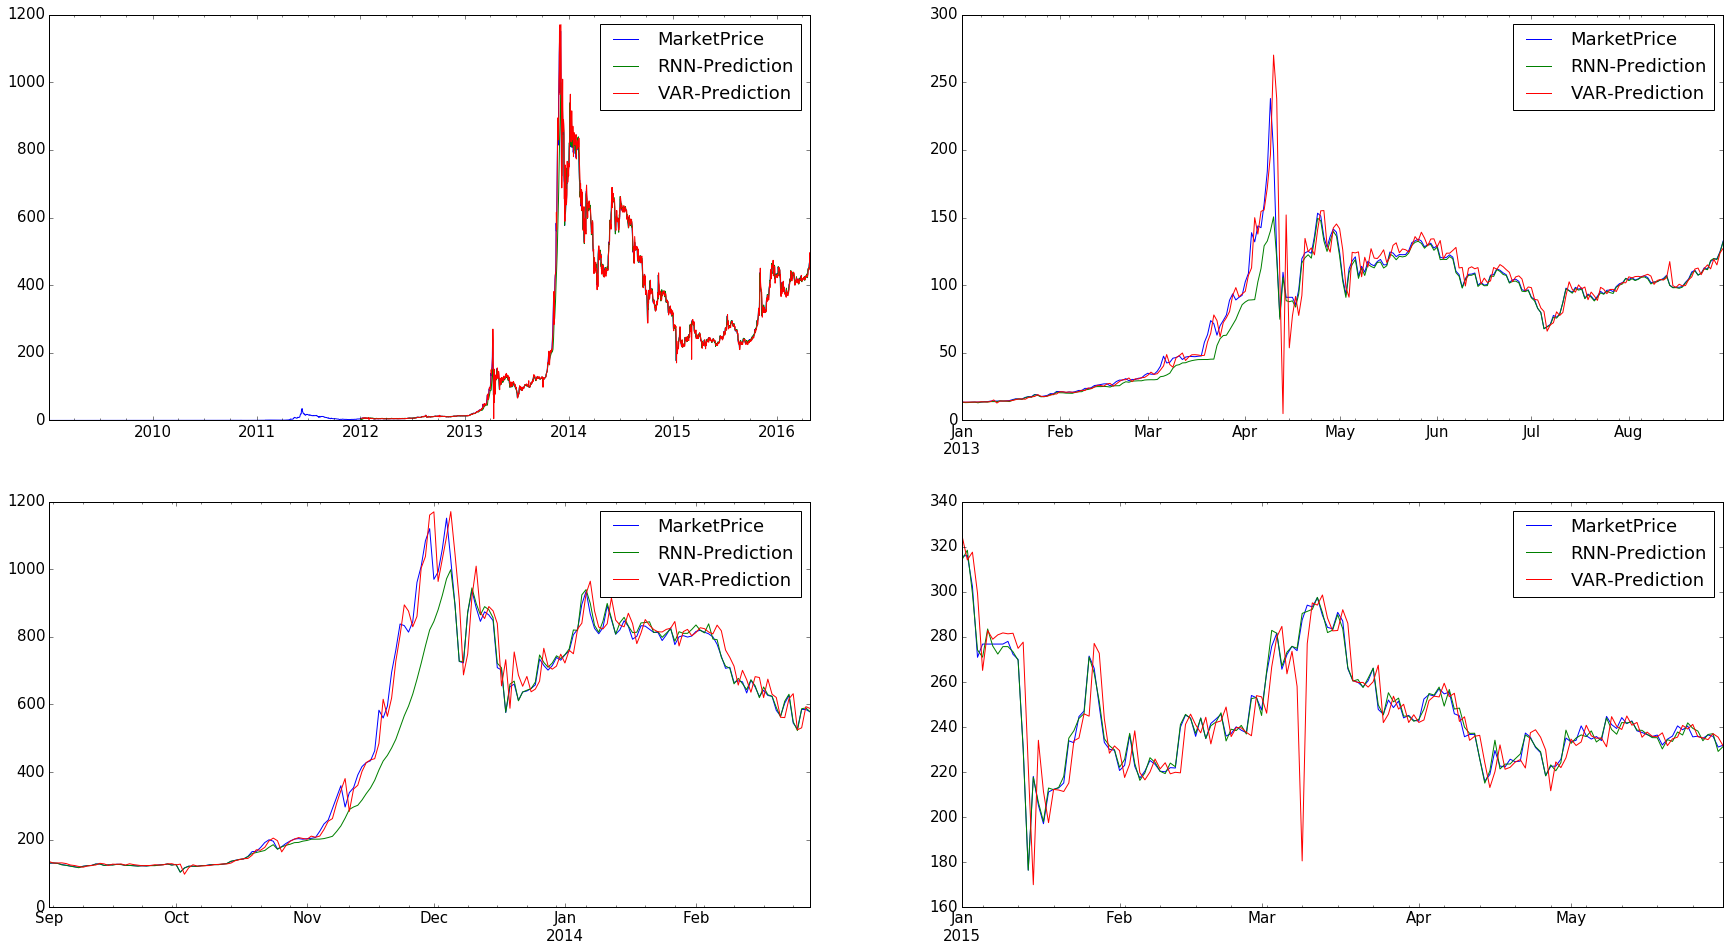
\includegraphics[width=1\linewidth]
    {gfx/predictions}}
  \caption{Predictions models and \textit{MarketPrice} true values in
    the same chart.}
  \label{fig:predictions}
\end{figure}

% TODO:
[[[Write about the accuracy measures used, their mathemathical expresion.
Talk about the properties of the measure.]]]

\begin{table}[bth]
  \myfloatalign
  \tiny
  \begin{tabularx}{\textwidth}{Xcc} 
    \toprule
    \tableheadline{Measure Type} & \tableheadline{RNN Value} & \tableheadline{VAR Value} \\
    \midrule
    Mean Absolute Error (MAE) & $5.4$ & $8.57$ \\
    Mean Squared Error (MSE) & $638.55$ & $367.82$ \\
    Mean Absolute Percentage Error (MAPE) & $3.19$ & $3.46$ \\
    Theil's U statistic & $0.47$ & $0.03$ \\

    \bottomrule
  \end{tabularx}
  \caption{Forecast accuracy measures}
  \label{tab:forecast-accuracy-measures}
\end{table}


[[[Analysis]]]

\begin{figure}[bth]
  \myfloatalign
  {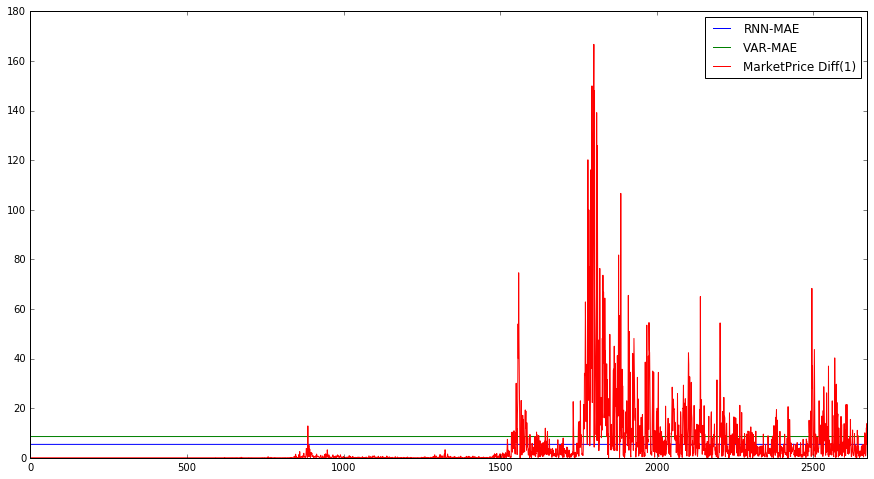
\includegraphics[width=1\linewidth]
    {gfx/comparison-mae-with-diffs}}
  \caption{Comparison of VAR-MAE value with \textit{MarketPrice} first
    difference values.}
  \label{fig:comparison-mae-with-diffs}
\end{figure}

\begin{figure}[bth]
  \myfloatalign
  {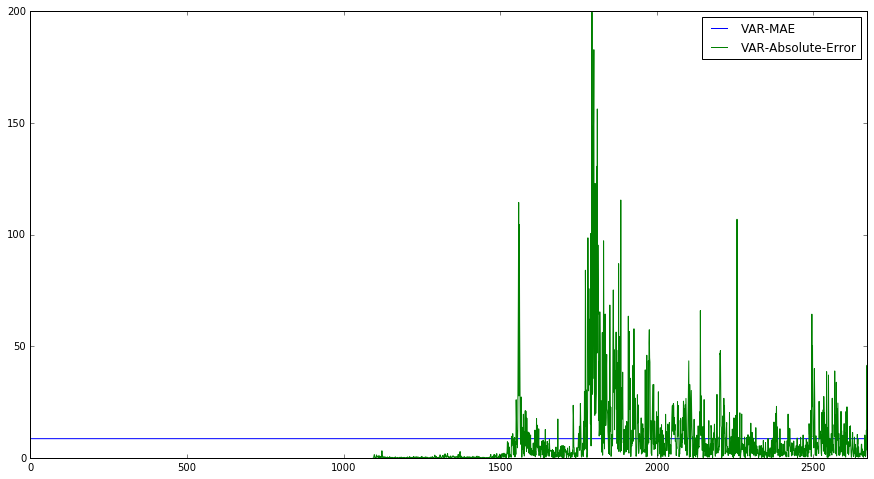
\includegraphics[width=1\linewidth]
    {gfx/comparison-var-mae-with-var-absolute-error}}
  \caption{Comparison VAR-MAE with  absolute VAR errors.}
  \label{fig:comparison-var-mae-with-var-absolute-error}
\end{figure}

\begin{figure}[bth]
  \myfloatalign
  {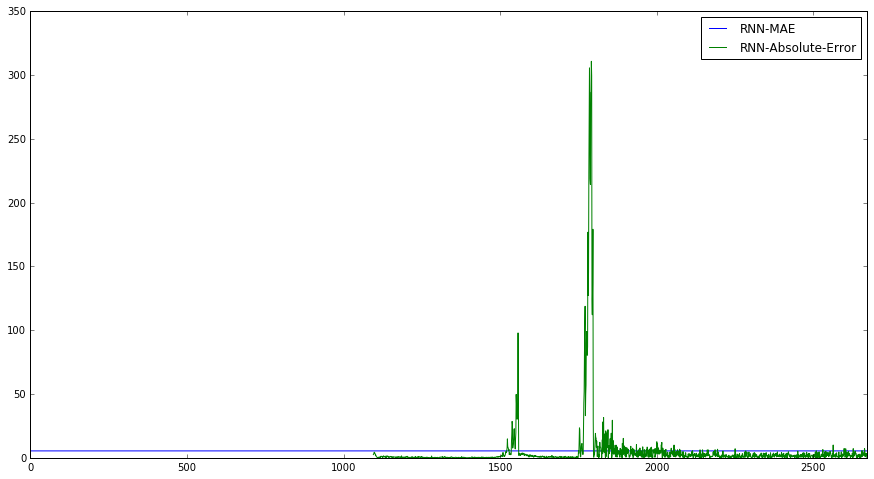
\includegraphics[width=1\linewidth]
    {gfx/comparison-rnn-mae-with-rnn-absolute-error}}
  \caption{Comparison RNN-MAE with  absolute RNN errors.}
  \label{fig:comparison-var-mae-with-var-absolute-error}
\end{figure}

\begin{figure}[bth]
  \myfloatalign
  {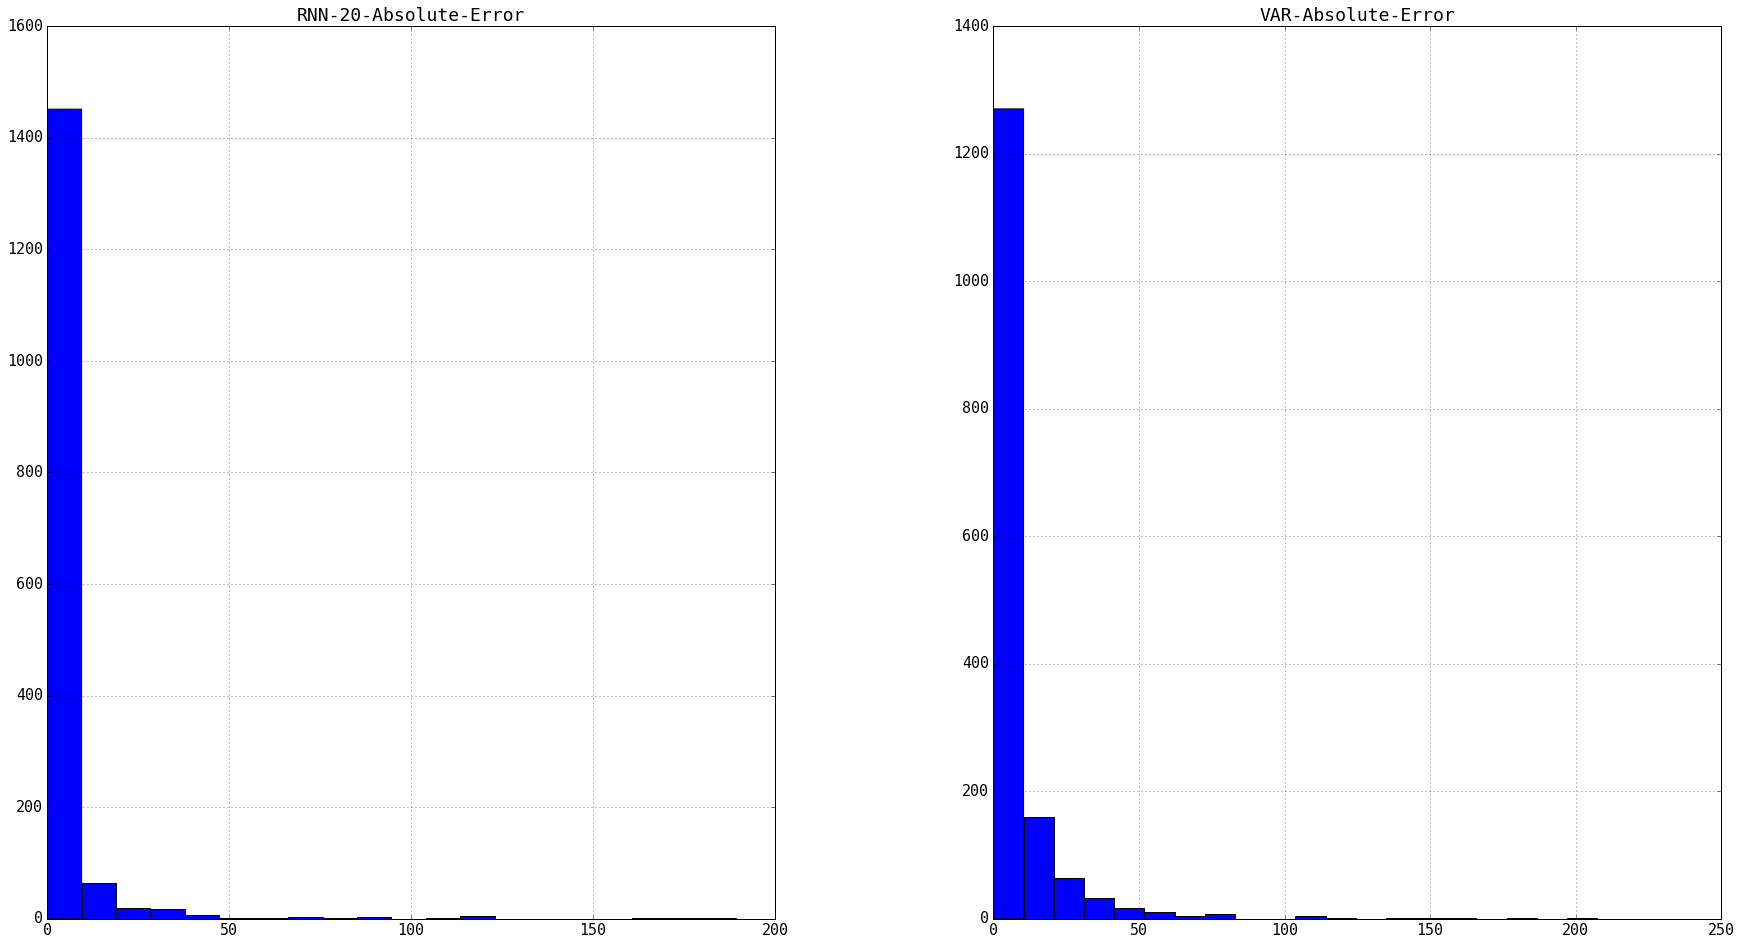
\includegraphics[width=1\linewidth]
    {gfx/comparison-histogram-prediction-errors}}
  \caption{Histogram of RNN absolute errors and VAR absolute errors.}
  \label{fig:comparison-histogram-prediction-errors}
\end{figure}

%---------------------------------------------------------------------
%---------------------------------------------------------------------
%---------------------------------------------------------------------

%\enlargethispage{2cm}

%------------------------------------------------

%%% Local Variables:
%%% mode: latex
%%% TeX-master: "../main"
%%% End:
